% !TeX spellcheck = en_GB
\chapter{Use of Physical Behaviours for Trust Assessment} \label{ch:physical_trust}
\lhead{Chapter \thechapter. \emph{Physical Trust Assessment}}

\section{Physical Behaviours for Trust}\label{sec:physbev}

\subsection{Physical Metrics}
The aim of any \gls{tmf} is to constrain the operation of a system such that any ``trusted'' behaviour is inherently ``correct'' behaviour; by monitoring \gls{plr}, delay, and throughput etc. 
In the communications domain, \glspl{tmf} aim to optimise the efficiency of these aspects of the networks performance.

Looking at the physical domain, the question becomes ``What characteristics of the nodes operations require constraint or optimisation, and what information is exposed to assess those?''.

Fundamentally, the physical information available (or at least, is reasonable to assume) is simple positional and velocity information reported by the nodes itself.
These assessments could be augmented with the use of sonar or visual tracking at short distances, or through time-of-flight positioning, but in the marine environment, both of these are difficult to accomplish and maintain consistently.

As for what characteristics of operations require optimisation, an assumption can be made that the primary threat is of a masquerading or damage of a node by a competent attacker, i.e.~ a physical \gls{tmf} should identify nodes that are behaving oddly. 
Additionally, and in a less threatening manner, an additional aspect to optimise for is efficiency of mobility and communication, i.e.~ maintaining relative proximity to lower communications energy costs, and minimise expensive or ``thrusty'' course corrections.

Therefore, based on a fuzzy incomplete knowledge of the position and velocities of fleet/team members over time, designed around the REMUS 100 AUV’s Kinematics, three primary initial metrics are arrived at:
\pagebreak
\begin{enumerate}
\item \emph{\acrfull{indd}}, a second order measure of the variation in the average distances between nodes in a squad
\item \emph{\acrfull{inhd}}, similar to \gls{indd} but based on instantaneous unit velocity, i.e. the direction of travel
\item \emph{Node Speed}, looking at the variability of through-the-water speed of each node in the squad with respect to the observable squads’ speeds.
\end{enumerate}
Using these metrics, appropriate behaviour within a dynamic fleet can be assessed dynamically and in a decentralised fashion.
%\todo{ADD MAYBE: Do more physical metrics (Theres lots more in bounous.Analyses.Metrics), this might be better chucked in the appendix }

These physical metrics are used to encompass the relative distributions and activities of nodes within the network. 
As such, these metrics completely encapsulate and abstract the physical behaviour of any node, potentially performing any misbehaviour.
Given that local nodes within the team are aware of the reported positions and velocities of their neighbours, it is believed that this is a reasonable set of metrics to establish the usefulness of physical metrics of trust assessment.

Additional metric constructions may be more suitable for certain contexts, platforms or operations, however these were selected in collaboration with UK DSTL and NATO CMRE as suitable, generic, assessments, viable on most current platforms in most current deployment schemes\footnote{An additionally prototyped metric was Reported Position Deviation which used a per-node Enhanced Kalman filter based ``god view'' estimator that constructed positional models based on highly accurate timing and time-of-flight modelling for non-linear channel paths to predict the movements of squad members and report discrepancies against their periodic positional updates (assumed to be part of a normal broadcast protocol), however this investigation is outside the scope of this current work}.

\begin{align}
  INDD_{i,j} &= \frac{|P_j - \sum_x \frac{P_x}{N}|}{\frac{1}{N}\sum_x \sum_y{|P_x - P_y| (\forall x \neq y)}}\\
  INHD_{i,j} &= \hat{v} \vert v= V_j - \sum_x{\frac{V_x}{N}}\\
  V_{i,j} &= |V_j|
\end{align}

Where $i$ and $j$ are indices denoting the current observer node and the current observed node respectively; $x$ is a summation index representing other nodes in the observers region of concern; $P_{j}$ is the $[x,y,z]$ absolute position of the observed node (relative to some coordinated origin point agreed upon at launch) and $V_{j}$ is the $[x,y,z]$ velocity of the observed node.

Thus, the metric vector used for the physical-trust assessment from one observer node to a given target node is;

\begin{equation}
  X_{i,j}=\{\text{INDD}_{i,j}, \text{INHD}_{i,j},, V_{i,j}\}
  \label{eq:phys_vector}
\end{equation}
At each time-step, each node will have a separate $X$ assessment vector for each node it has observed in that time. 
Ergo the fleet or team as a whole will have $N\times N-1$ assessment vectors at each timestep.

\subsection{Physical Misbehaviours}

Misbehaviours in the communications space is heavily investigated area in \glspl{manet}~\cite{Konate2011,Wang2009,Chen2014a,Mitchell2014}, but attacks and misbehaviours in the physical space are far less explored. 
Both in terrestrial and underwater contexts, as \gls{manet} applications expand and become increasingly \emph{de rigueur}, the impacts of physical or operational misbehaviour become increasingly relevant. 
As in the communications space, the primary drivers of any ``misbehaviour'' come under two general categories; selfish operation or malicious subterfuge.
Autonomous \glspl{manet} in general rely (or are at least, most effective) when all nodes operate fairly, be that in terms of their bandwidth sharing, energy usage, routing optimality or other factors. 
Physically, if a node is being ``selfish'', it may preferentially move to the edge of a network to minimise it's dynamic work allocation, or depending on it's intent, may insert itself into the centre of a network to maximise it's ability to capture, monitor, and manipulate traffic going across the network. 
In the context of a secure operation (or one that's assumed to be secure), there is also the opportunity for capturing a legitimate node and replacing it with a modified clone.
Assuming a highly capable outside actor and a multi-channel communications opportunity, there is also the possibility of a node appearing to ``play along'' with the crowd that occasionally breaks rank to route internal transmissions to a outside agent.
In the underwater context this may mean an AUV following the rest of a team along a survey path and occasionally ``breaking surface'' to communicate to a malicious controller using a secondary communications link such as WiFi or satcomms.
Alternatively, if an inserted node is not totally aware of a given mission parameter, such as a particular survey or waypointing path, it may simply follow along, hoping not to be noticed.

In all these cases, such behaviour involves some element of behaving differently from the rest of the team, however, there are other cases where such individual ``deviance'' is observed; where a node is in some kind of mechanical ``failure state''.
In the underwater context, this could be damage to the drive-train or navigation systems, causing it to lag behind or consistently drift off course. 
An ideal physical trust management system would be able to differentiate between both ``malicious'' behaviours and ``failing'' behaviours.

To investigate this hypothesis, we create two ``bad'' behaviours; one ``malicious'', where a cloned node is unaware of the missions' survey parameters and attempts to ``hide'' among the fleet, and a ``failing'' node, with an impaired drive train, increasing the drag force on the nodes movement.
These two behaviours are designated \emph{Shadow} and \emph{SlowCoach} respectively.
\pagebreak
\section{Simulation and Validation}\label{sec:sim_and_valid}

\subsection{Simulation Background}

\begin{figure}
	\centering
	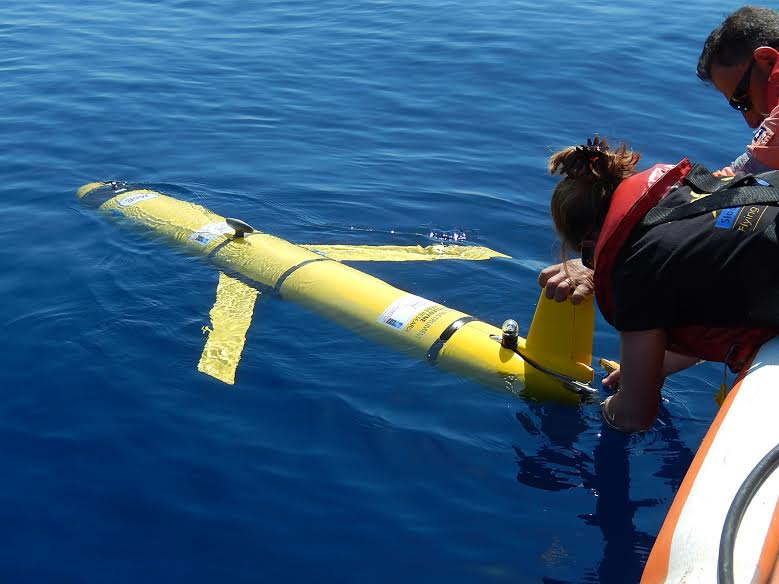
\includegraphics[width=0.40\textwidth]{img/glider.jpg}
	\caption{REMUS 100 Craft deployed at CMRE, La Spezia, Italy}
	\label{img:remus}
\end{figure}

Simulations were conducted using a Python based simulation framework, SimPy~\cite{Mueller2003SimPy}, with a network stack built upon AUVNetSim~\cite{Miquel2008}, with transmission parameters taken from and validated against~\cite{Stojanovic2007} and~\cite{Stefanov2011}.
For the purposes of this chapter, this network is used for the dissemination of node location information, assuming suitable compression of internally assumed location data compressed into one 4096 bit acoustic data frame, with the network overall emitting approximately 10 frames a minute.
Node kinematics are modelled on REMUS 100 \glspl{auv} (\autoref{img:remus}), based on limits and core characteristics given in~\cite{Mcewen2001,Milgram2001,Samad2011}.\footnote{While the hydrodynamics of the control surfaces of the \glspl{auv} are not modelled in this case, axial drag is modelled as a resistive inertial force on the craft.}
These limits are given in Table~\ref{tab:mobility_sysconstraints}.


\begin{table}
  \caption{REMUS 100 Mobility Constraints as applied in simulation} \label{tab:mobility_sysconstraints}
  \begin{center}
    \setlength{\tabcolsep}{8pt}
    \begin{tabular}{lcc}
      \toprule
      Parameter & Unit & Value \\
      \midrule
      Length & $m$ & 5.5\\
      Diameter & $m$ & 0.5\\
      Mass & $kg$ & 37 \\ 
      Max Speed & $ms^{-1}$ & 2.5\\
      Cruising Speed & $ms^{-1}$ & 1.5\\
      Max X-axis Turn & $^{\circ} s^{-1}$ & 4.5\\
      Max Y-axis Turn & $^{\circ} s^{-1}$ & 4.5\\
      Max Z-axis Turn & $^{\circ} s^{-1}$ & 4.5\\
      Axial Drag Coefficient ($c_d$) & NA & 3\\
      Cross Section Area & $m^2$ & 0.13\\
      \bottomrule
    \end{tabular}
    \setlength{\tabcolsep}{6pt}
  \end{center}
\end{table}

\subsection{Node Control Modelling}

In our investigation, we use the example of a Port Protection scenario, where a team of six \glspl{auv} are tasked with surveying a simplified harbour; in this case a 1kmx1kmx100m cuboid volume.
This is accomplished through a distributed way point system where by the team overall must ``check'' several points around the exterior and interior of this volume in reasonable time.
In addition to this, there is a reasoned requirement for both collision avoidance and a pressure for the fleet to maintain communications distance.

These are encapsulated as three heuristic rules; Cohesion, Repulsion and Alignment.
\begin{align}
  F_{j,C}=& F_+\left(p_j, \frac{1}{N}\sum\limits_{\forall i \ne j}^N{p_i}, d_{max}\right)\label{eq:fa}\\
  F_{j,R}=& \sum\limits_{\forall i \ne j}^N F_-\left(p_j, p_i, d_{max}) \big| d_{max}>\|p_i-p_j\|\right)\label{eq:fr}\\
  F_{j,A}=& \frac{1}{N}\cdot\left(\sum\limits_{\forall i \ne j}^N \hat{v_i}\right)\label{eq:fc}
\end{align}
Where $F$'s are force-vectors applied to the internal guidance of the \gls{auv}, $F_{j,C}$ representing Cohesion, $F_{j,R}$ representing Repulsion, and $F_{j,A}$ as Alignment: $F_+$ is a scaled vector attraction function, and $F_-$ is an equivalent repulsion function
\begin{align}
  F_+(p^a, p^i)=&(\widehat{p^a-p^i}) \times \frac{|p^a-p^i|}{d}\\
  F_-(p^r, p^i)=&(\widehat{p^i-p^r}) \times \frac{|p^r-p^i|}{d}
\end{align}

In essence, the fleet is simultaneously attracted to its current target waypoint as well as a lesser attraction to the centre of the fleet to retain communications.

\begin{figure*}
  \centering
  \begin{subfigure}[t]{0.3\textwidth}
    \centering
    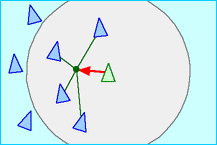
\includegraphics[width=\textwidth]{flocking_cohesion}
    \caption{Cohesion}
  \end{subfigure}
  \begin{subfigure}[t]{0.3\textwidth}
    \centering
    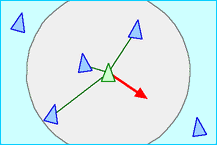
\includegraphics[width=\textwidth]{flocking_separation}
    \caption{Repulsion}
  \end{subfigure}
  \begin{subfigure}[t]{0.3\textwidth}
    \centering
    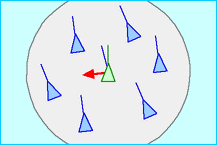
\includegraphics[width=\textwidth]{flocking_alignment}
    \caption{Alignment}
  \end{subfigure}
  \caption{Visual representation of the basic Boidean collision avoidance rules used}
  \label{fig:boids}
\end{figure*}


\subsection{Standards of Accuracy}\label{sec:standards}

The key question of this chapter is to assess the advantages and disadvantages of utilising trust from the physical domain. 

It is important to clarify what is meant by ``effective'' in this case; the ``effectiveness'' of any trust assessment framework is taken as consisting of several parts, the \emph{accuracy} of detection and identification of a particular misbehaviour, the \emph{complexity} of such analysis, including any specific training required, and the \emph{differentiability} of behaviours using given metrics.

In this case we are particularly interested in the accuracy of detection and identification of malicious / failing behaviours, and as such are looking at three key characteristics of accuracy; true detection accuracy (what percentage of ``bad'' behaviours are detected at all); false positive rates (what percentage of ``control'' behaviours are detected as being ``bad''); and misidentification rates (how many instances of one bad behaviour are mischaracterised as the other and vice versa.

As such we have three primary questions to answer to establish if these metrics are useful: 
How accurate are these metrics in being able to easily differentiate between Normal and Abnormal behaviours in terms of True-Positive and False-Positive rates?
What differentiation of response, if any, is there between the stated abnormal behaviours?
Can a simple classification be built to characterise these differentiations of response, and what is it's True-Positive/False-Positive accuracy?


\subsection{Analysis}
Having established the metrics under investigation, 64 simulation runs are executed for each scenario (i.e.\ one node ``Maliciously'' following the fleet with no mission information (Shadow), one ``Failing'' node with simulated drive train issues (Shadow), and one baseline control scenario where all nodes are behaving appropriately (Control).
Each of these simulated missions last for an hour, matching realistic deployment times based on current MOD/NATO operations\cite{Bolster2014a}.

\subsubsection{Metric Cleaning}
In order to assess the viability of using the previously discussed metrics, the raw motion paths recorded by the simulation are fed into an analysis pipeline aimed at abstracting the instantaneous observed values into derived deviations from ``normal'' behaviour in the team.

\begin{align}
  d_{i,j}^{m,t} &= x_{i,j}^{m,t} - \frac{\sum_k x_{i,k}^{m,t}}{|M|}\label{eq:d}\\
  \alpha_{i,j}^{m,t} &= | \frac{d_{i,j}^{m,t}}{\sigma{d_{i,j}^{m,t}}}|\label{eq:dd}
\end{align}

Where $i$ and $j$ are indices denoting the current observer node and the current observed node respectively; $x$ is a summation index representing other nodes in the observers region of concern; $X$ is the vector of metrics from~\ref{eq:phys_vector}; $d$ is an intermediate value of the distance of a given observation from the mean, and $\alpha$ is a resulting normalised response value in terms of it's deviation from the mean.

\subsubsection{Behaviour Detection and Classification}
A simple misbehaviour detection is to apply Dixon's Q-test~\cite{Dean1951} to the resultant $\sum\alpha$ values for each node for each metric for each run establishing if a ``misbehaving node'' exists in a given run, and if so, attempt to identify that misbehaving node. 
For our initial investigation we will use a Confidence Interval of $95\%$.

Our initial hypothesis is that by using observations of the previously stated physical metrics, that we will be able to detect and identify misbehaviours.
Within that context, this Confidence Interval indicates that we would expect only a $5\%$ chance that any run or node identified using the Q-test to \emph{not} be a misbehaving run/node.
Further, due to the range of metrics available, by applying the Q-test on a per-metric basis, we can use the ``votes'' of each metric as a simplified consensus classifier.
This classifier may allow us to characterise some aspect of a given misbehaviour in terms of metrics it heavily impacts, and those that are less affected, finding some differentiating-limit between certain behaviours using certain metrics.


\subsubsection{Operational Performance Metrics}
While not the focus of this chapter, we are also concerned with the impact of these misbehaviours on the mission efficiency of the team overall.
We monitor this in three main measurements; the ``speed'' of the fleet in terms of how many of it's port-protection way points it successfully approaches and passes, the total energy used for communications, and the average end-to-end delay in the acoustic network.
We would expect that any misbehaviour in positioning will incur some loss of efficiency, whether it is the fleet being slowed down by a straggler attempting to catch up or of a node moving in an unexpected fashion dragging the team temporarily off course.
Given that in acoustic communications, transmission is energetically expensive while reception is not, and while physical misbehaviours will not impact the amount of offered load on the network, collisions induced by uneven distribution of nodes should have a small but measurable effect on energy used for packet reception.

\section{Results and Discussion}
Fig.~\ref{fig:metric_values} shows the raw metric values (vertically) from one run of each behaviour (horizontally), starting with the Control case, where all node are behaving properly with Alfa as the misbehaving node in the remaining cases.
It clear that using the (unitless) \gls{indd} and \gls{inhd} metrics, Alfa is the outlier and other, fairly behaving, nodes are all consistent in their metric values.
This outlier-response is not nearly as clear in the Speed metric case (bottom row of Fig.~\ref{fig:metric_values}).
This would be expected considering the cumulative factor of increasing distance between nodes if a given node is ``lagging'' behind.

From a behaviour-perspective, it appears that the Shadow behaviour is creating the largest, most obvious deviations.

\begin{figure*}
  \centering
  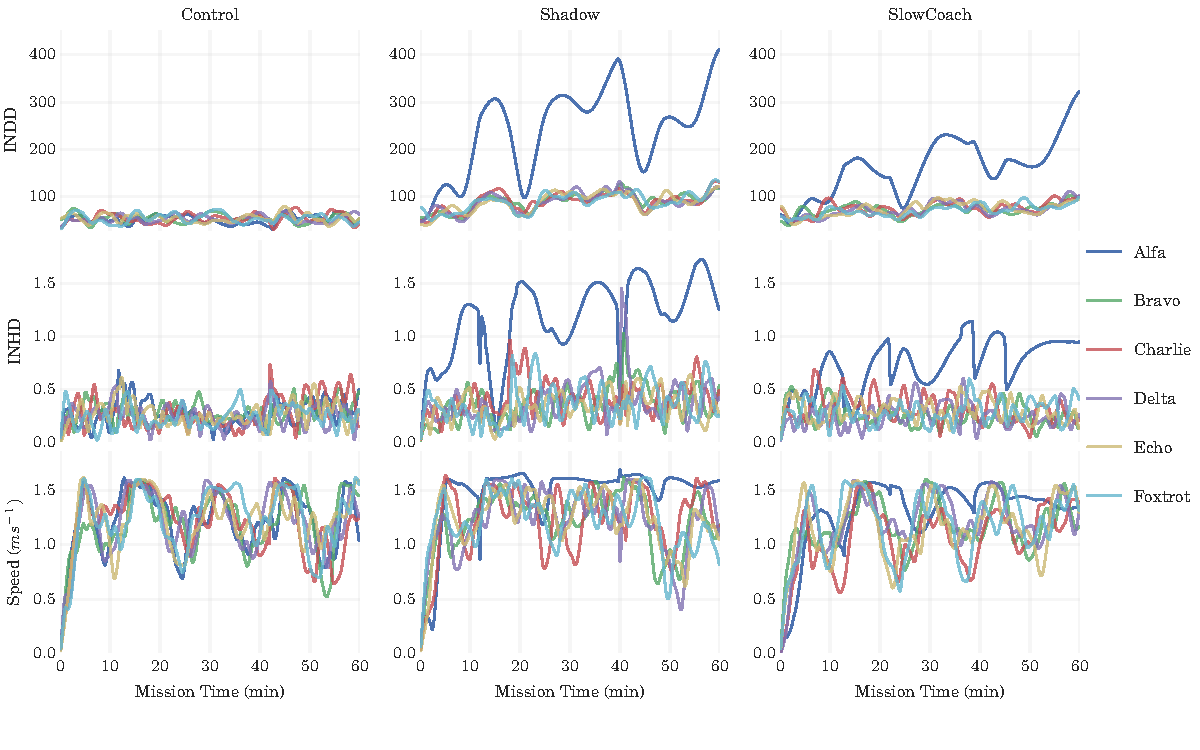
\includegraphics[width=\textwidth]{Metric_Values}
  \caption{Observed Metric Values for one simulation of each behaviour ($x_{i,j}^{m,t}$ from \eqref{eq:d})}
  \label{fig:metric_values}
\end{figure*}

\begin{comment}
\begin{figure*}
  \centering
  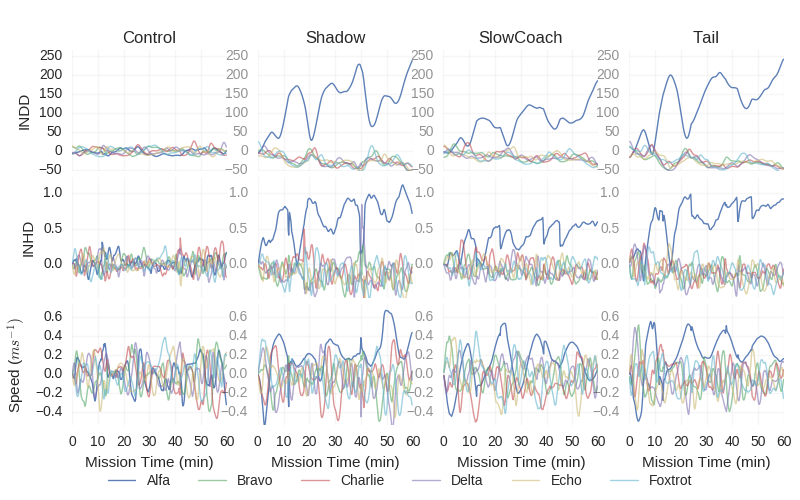
\includegraphics[width=\textwidth]{Metric_Deviation}
  \caption{\emph{Unnecessary but included for draft discussion} Observed Metric Values for one simulation of each behaviour ($d_{i,j}^{m,t}$ from Fig.~\ref{fig:workflow})}
\end{figure*}
\end{comment}

In Fig.~\ref{fig:deviance_values} the metric values are normalised as per \eqref{eq:dd}.
This has highlighted the outlying-characteristic of \gls{indd} and \gls{inhd}; largely eliminating the other nodes-responses.
In the Speed response of Fig.~\ref{fig:deviance_values}, the Speed metric is not obviously highlighting any significant misbehaviours in that metric. 

\begin{figure*}
  \centering
  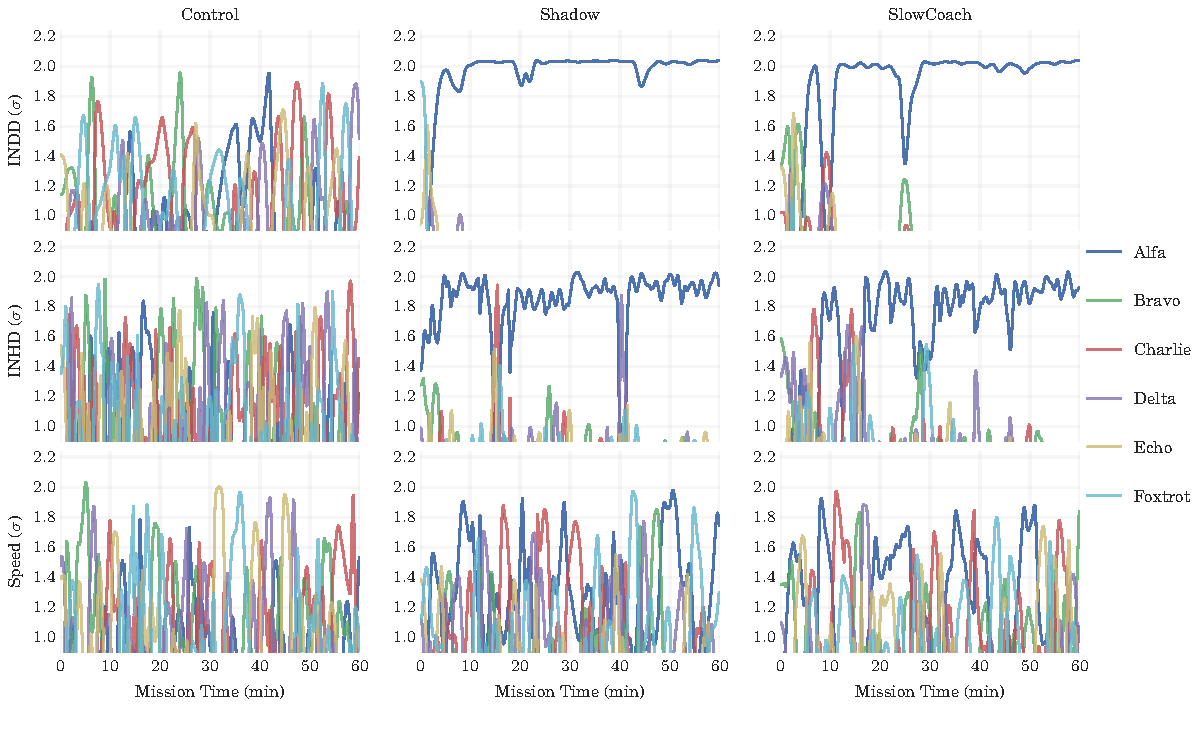
\includegraphics[width=\textwidth]{Metric_Sigma_Deviance}
  \caption{Normalised Deviance values from one simulation of each behaviour ($\alpha_{i,j}^{m,t}$ from \eqref{eq:dd})}
  \label{fig:deviance_values}
\end{figure*}

From Fig.~\ref{fig:summedsigmabar}, it appears that Speed is being significantly affected by the differing behaviours, but much less so than \gls{indd}/\gls{inhd}.  

\begin{figure*}
  \centering
  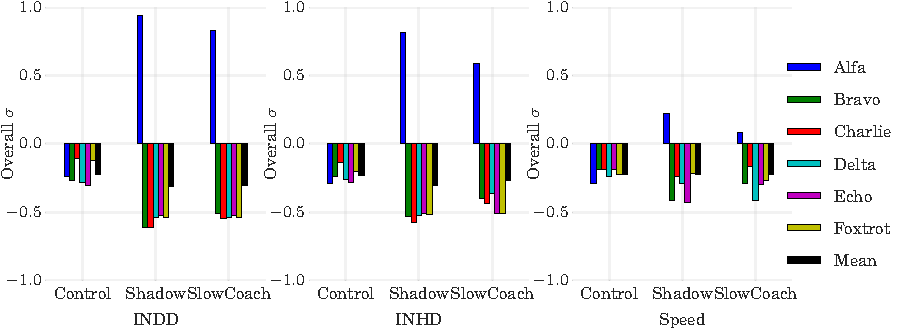
\includegraphics[width=\linewidth]{summedsigmabar}
  \caption{Per-Node-Per-Run deviance for each metric, normalised in time ($\sum\alpha/T$)}
  \label{fig:summedsigmabar}
\end{figure*}

\subsection{Detection of Misbehaviours}
It has been demonstrated by graphical result that from the initial metrics set, \gls{indd} and \gls{inhd} do appear to accurately and obviously identify the malicious node in the case that there is one. 
Using the deviance normalisation presented in \eqref{eq:dd}, clear, almost contiguous areas under the Alfa-values are observed in Fig.~\ref{fig:deviance_values} in the Shadow and SlowCoach misbehaviours.
Further, from Fig.~\ref{fig:summedsigmabar}, it is shown that while it is nowhere near as ``clear'' as the deviance in \gls{indd} and \gls{inhd}, that the Speed metric is still registering a statistically significant deviation in both misbehaviours, and that the difference between the deviances in Speed may indicate a way to analytically differentiate between the two misbehaviours.

To investigate how this would relate to the ability to blindly detect misbehaviours, the Q-test is applied to $\Sigma\alpha$ results as used in Fig.~\ref{fig:summedsigmabar}, to attempt to correctly establish:
\begin{enumerate}
  \item if a node is misbehaving and
  \item which node is misbehaving
\end{enumerate}

As such, the ``correctness'' rule for assessing this strategy is that, in misbehaving cases, the Q-tests should return Alfa (otherwise a ``Fail'' is recorded), and in the Control case, the Q-test should assert that there are no obvious outliers, (otherwise a ``Fail'' is recorded again).
In Table~\ref{tab:overall_stats}, the Null case (Control behaviour) is correctly identified 92\% of the time.
The ``malicious'', Shadow misbehaviour is detected and identified 98\% of the time, and the ``failing'', SlowCoach misbehaviour is identified just 79\% of the time. 
These values match our intuition from Figs.~\ref{fig:metric_values} and~\ref{fig:deviance_values}.

\begin{table}
  \caption{Overall Q-Test Outlier Correct Detection Accuracy}
  \centering
\begin{tabular}{lll}
\toprule
Behaviour &  Mean &   Std. \\
\midrule
Control   & 0.927 & 0.261 \\
Shadow    & 0.979 & 0.144 \\
SlowCoach & 0.792 & 0.408 \\
\bottomrule
\end{tabular}
  \label{tab:overall_stats}
\end{table}

We can investigate this further by looking at the ``correctness'' of the assessments of each metric individually (Table~\ref{tab:per_metric_stats}).
In both misbehaviours, \gls{indd} and \gls{inhd} correctly identify Alfa as the misbehaver 100\% of the time. 
However, they misidentify a potential misbehaviour in the Control case 13\% and 7\% of the time respectively.
Meanwhile, Speed correctly identified the Control case 97\% of the time, and the Shadow case 94\% of the time, but missed the SlowCoach behaviour 63\% of the time. 
This result is surprising on the face of it, as SlowCoach is a misbehaviour that is exclusively about individual node speed and conceptually should have had a much larger impact on the simple Speed metric.
However, the collaborative nature of the collision avoidance system, and the existing limits on node kinematics from Table~\ref{tab:mobility_sysconstraints} are masking this impact. 

\begin{table}
  \caption{Per-Metric Q-Test Outlier Detection Accuracy}
  \centering
\begin{tabular}{lllll}
\toprule
{} & Behaviour &  INDD &  INHD & Speed \\
\midrule
Mean & Control & 0.875 & 0.938 & 0.969 \\
     & Shadow & 1.000 & 1.000 & 0.938 \\
     & SlowCoach & 1.000 & 1.000 & 0.375 \\
Std & Control & 0.336 & 0.246 & 0.177 \\
     & Shadow & 0.000 & 0.000 & 0.246 \\
     & SlowCoach & 0.000 & 0.000 & 0.492 \\
\bottomrule
\end{tabular}
  \label{tab:per_metric_stats}
\end{table}

\subsection{Identification of Misbehaviours}
Having established the ability of \gls{indd}, \gls{inhd} and Speed to all detect physical misbehaviour to a statistically significant level, and having shown that there is a demonstrable difference in response to different misbehaviours, we return to the last question from Sec.~\ref{sec:standards}; can a simple classifier based on a subset of our results be constructed, and can it be blindly applied to a new set of results successfully?

From~\eqref{eq:confidence}, the per-metric-per-behaviour ``Confidence'' in the relationship between a given metric deviance and each behaviour is established. It is hypothesised that this confidence can be used as a signature for that metric.

\begin{equation}
C_{i}^{m} = \Sigma_t\sigma_{i}^m * \frac{N-1}{\sum_{x\neq i}{\Sigma_t\sigma_{x}^m}}\label{eq:confidence}
\end{equation}

\begin{table}[h]
  \caption{Metric Confidence Responses for known behaviours~\eqref{eq:confidence}}
  \centering
\begin{tabular}{llrrr}
\toprule
{} & Behaviour &  INDD &  INHD &  Speed \\
\midrule
Mean & Control & 1.064 & 0.966 &  1.010 \\
     & Shadow & 4.059 & 3.374 &  2.098 \\
     & SlowCoach & 4.246 & 3.352 &  1.491 \\
Std & Control & 0.262 & 0.113 &  0.132 \\
     & Shadow & 0.398 & 0.436 &  0.206 \\
     & SlowCoach & 0.198 & 0.288 &  0.180 \\
\bottomrule
\end{tabular}
  \label{tab:confidence}
\end{table}

Having demonstrated that the Null case (All nodes behaving fairly) can be identified to a strong degree of accuracy, our classifier will continue to use the Q-test across all metrics for that case and concentrate of differentiating the Shadow and SlowCoach behaviours where they exist.

From Table~\ref{tab:confidence} it is clear that \gls{indd} and \gls{inhd} have similar responses to both misbehaviours, with significant standard deviations, but the response of the Speed metric is much more stable and discernible; across the range of training simulation runs.
In the SlowCoach behaviour, this Speed response centres around $1.5$, while the Shadow behaviour centres around $2.0$, with these centres being at least one standard deviation away from each other respectively.

Our generated classifier is formalised in~\eqref{eq:classifier}.

\begin{equation}
  C \rightarrow 
  \begin{cases}
    % Control
    Q^{95}(X) = \emptyset,& \text{Control}\\
    % Shadow
    Q^{95}(X) \neq \emptyset \land \text{Speed}^X \leq 1.75, & \text{Shadow}\\
    % SlowCoach
    Q^{95}(X) \neq \emptyset \land \text{Speed}^X > 1.75,& \text{SlowCoach}\\
  \end{cases}
  \label{eq:classifier}
\end{equation}

Applying this simplified classifier to a blind test set of simulations (of the same scale) gives surprisingly positive results as shown in Table~\ref{tab:classifier}, with greater than 90\% identification rates for both misbehaviours.
However, in the Null (Control) case we experience a false-positive rate of nearly 30\%, that is to say that in the case where there is no misbehaviour, 30\% of the time a node will be misidentified as misbehaving when it is not.

\begin{table}[h]
  \caption{Successful Identification rates on untrained results using~\eqref{eq:classifier}}
  \centering
  \begin{tabular}{lr}
    \toprule
    True Behaviour &  Probability of Correct Blind Identification \\
    \midrule
    Control        &                                        0.719 \\
    Shadow         &                                        0.906 \\
    SlowCoach      &                                        0.938 \\
    \bottomrule
  \end{tabular}
  %\begin{tabular}{lr}
\toprule
{} &  Probability of Correct Blind Identification \\
True Behaviour &                                              \\
\midrule
Control        &                                        0.719 \\
Shadow         &                                        0.906 \\
SlowCoach      &                                        0.938 \\
\bottomrule
\end{tabular}

  \label{tab:classifier}
\end{table}

If the rules of this classifier are loosened to require two deviating $Q^{95}(X)$ observations for detection of non-Control behaviours (i.e. multi-metric deviations), this false positive rate is eliminated while maintaining true-positive detection characteristics for misbehaviours.

\begin{equation}
C \rightarrow 
\begin{cases}
% Control
|Q^{95}(X)| \leq 1,& \text{Control}\\
% Shadow
|Q^{95}(X)| > 1 \land \text{Speed}^X \leq 1.75, & \text{Shadow}\\
% SlowCoach
|Q^{95}(X)| > 1 \land \text{Speed}^X > 1.75,& \text{SlowCoach}\\
\end{cases}
\label{eq:classifier_minority}
\end{equation}
\begin{table}[h]
  \caption{Successful Identification rates on untrained results using~\eqref{eq:classifier}, with outlier consensus checks}
  \centering
  \begin{tabular}{lr}
  	\toprule
  	True Behaviour &  Probability of Correct Blind Identification \\
  	\midrule
  	Control        &                                        1.000 \\
  	Shadow         &                                        0.906 \\
  	SlowCoach      &                                        0.938 \\
  	\bottomrule
  \end{tabular}
  %\begin{tabular}{lr}
\toprule
{} &  Probability of Correct Blind Identification \\
True Behaviour &                                              \\
\midrule
Control        &                                        1.000 \\
Shadow         &                                        0.906 \\
SlowCoach      &                                        0.938 \\
\bottomrule
\end{tabular}

  \label{tab:classifier_minority}
\end{table}

Given the simplicity of the applied classifiers, these are strongly positive results for the use of physical metrics for behaviour discrimination; with \gls{indd} and \gls{inhd} proving as strong and obvious ``canaries'' of misbehaviour, and Speed in this case proving a capable differentiator between conceptually close misbehaviours.


\subsection{Impacts of Misbehaviour on operational performance}
The anticipated ``small but measurable'' effects to communications performance and energy usage are indeed extremely small and within the bounds of statistical uncertainty.
One observation of merit was an observed 10\% increase in end-to-end delay in the case of the Shadow behaviour; this is due to the misbehaving node ``overshooting'' the mission way points and thus temporarily looking local connection to nodes on the opposite side of the fleet from it, causing retransmissions thus, delays.
As for physical efficiency, achievement rates were identical to within 2\% error on each run across all behaviours, and fleet distance varied by a similar margin.
It's possible that our selected behaviours were too unambitious in our impacts, and future work will have to investigate the impact of ``heavy-handed'' or destructive behaviours on the operational efficiency of autonomous networks.

\section{Conclusion}
In this chapter we have demonstrated that with current and on-the-horizon underwater localisation techniques, that in certain mobility models, that a set of relatively simple geometric abstractions (\gls{indd}, \gls{inhd}, and Speed), between nodes as part of an Underwater \gls{manet} can be used as a Trust Assessment and Establishment metric.

These metrics are application-agnostic and could potentially be applied in other areas of mobile autonomy such as \gls{auv} operations and Autonomous Vehicular Networks.

We show, using a Port-Protection way point scenario built upon a Boidian collision prevention behaviour that in a simulated underwater environment, the outputs of these metrics can be used to detect and differentiate between exemplar malicious behaviour and potential failure states.

This verification further supports the assertions the authors have made previously that it is practical to extend Trust protocols such as \gls{mtfm}~\cite{Guo2012} to include metrics and observations from the physical domain as well as those from the communication domain\cite{Bolster2014}.
In the next chapter, this combination of physical and ``logical'' information is explored to establish if it further supports the decentralised and distributed establishment of observation based Trust.

%%%%%%%%%%%%%%%%%%%%%%%%%%%%%%%%%%%%%%%%%%%%%%%%%%%%%%%%%%%%%%%%%%%%%%%%%%%%%%%
